\chapter{Two-dimensional Steady State problems}
\section{Overview}
\section{Separation of variables Method}
\begin{example}
\textcolor{blue} {\emph{Refer to tutorial HW\_1\_MMATICA.nb, and Ch. 3, P. 134.}}
A two-dimensional rectangular plate length and width is $L=2$,$W=1$, and on one 
boundary temperature $T_2=150~K$, other three boundaries $T_2=50~K$. The square 
is in steady state, what is the temperature at position $x=1$ and $y=0.5$?
Sketch the temperature distribution. (As shown in figure \ref{fig:3:1})
\begin{figure}[h!]
  \centering
    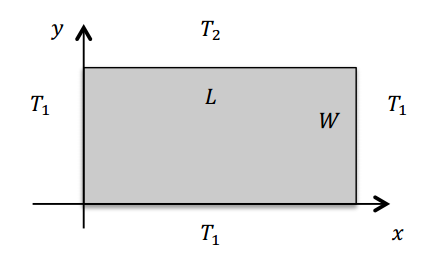
\includegraphics[scale=0.8]{figures/ch3/1}
    \caption{}
    \label{fig:3:1}
\end{figure}
\end{example}
\begin{solution}
To simplify the solution, use below transformation
$$\theta=\frac{T-T_1}{T_2-T_1}$$
According to heat diffusion equation, the two-dimensional, steady state with no internal heat generation equation is 
$$\frac{\partial^2 T}{\partial x^2}+\frac{\partial^2 T}{\partial y^2}=0$$
the transformed differential equation is then
$$\frac{\partial^2 \theta}{\partial x^2}+\frac{\partial^2 \theta}{\partial y^2}=0$$
Since the equation is second order in both x and y, two boundary conditions are needed for each of the coordinates, they are
$$\theta(0,y)=0,\text{and} \theta(x,0)=0$$
$$\theta(L,y)=0,\text{and} \theta(x,W)=1$$
The $\theta(x,y)$
The is Plot the 3D sketch of the temperature distribution in the rectangular
$$\theta(x,y)=\frac{2}{\pi}\sum\limits_{i=1}^\infty 
\frac{(-1)^{n+1}+1}{n}\sin{\frac{n\pi x}{L}}
\frac{\sinh{n\pi y/L}}{\sinh{n\pi W/L}}
$$
The plot of the 3D sketch of the temperature distribution in the rectangular is shown as Figure \ref{fig:3:2}
\begin{figure}[h!]
  \centering
    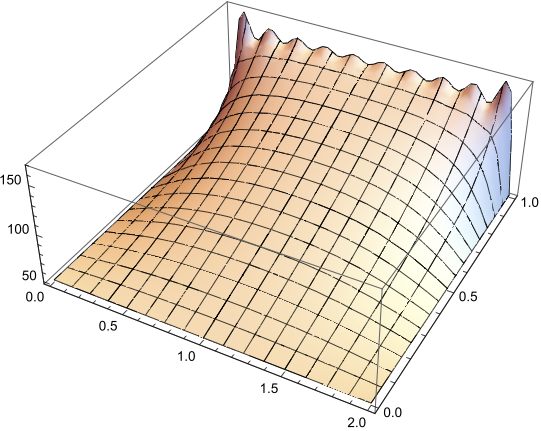
\includegraphics[scale=0.2]{figures/ch3/2}
    \caption{}
    \label{fig:3:2}
\end{figure}
\end{solution}


